\justifying
\chapter{Introduction and Background Research}

% Introduction
% Related Works
    % Evaluation

% Join spectrums into one section

% You can cite chapters by using '\ref{chapter1}', where the label must
% match that given in the 'label' command, as on the next line.
\label{chapter1}

% Sections and sub-sections can be declared using \section and \subsection.
% There is also a \subsubsection, but consider carefully if you really need
% so many layers of section structure.

%<A brief introduction suitable for a non-specialist, {\em i.e.} without using technical terms or jargon, as far as possible. This may be similar/the same as that in the 'Outline and Plan' document. The remainder of this chapter will normally cover everything to be assessed under the `Background Research` criterion in the mark scheme.>
\section{Introduction}
Ocean surface simulation \ref{fig:ocean_simulation} is a field of computer graphics that aims to create realistic representations of the ocean surface.
It is an important area of research as it has a wide range of applications, including video games, movies.
In video games it used for interactivity and visual appeal, while in movies it is used for visual appeal. 

There are many techniques that have been developed to simulate ocean surfaces, from the simple algorithms as 
sum of sines or Gerstner waves to more complex techniques such as particle simulations or Fast Fourier Transform (FFT) based Ocean \ref{fig:ocean_simulation}.

An essential aspect of ocean surface simulation is shading, which adds depth and realism to the rendered image. Two commonly used models for this purpose are Phong Shading and Physically Based Rendering (PBR). Phong Shading provides a balance between simplicity and visual quality, making it a popular choice for various applications. On the other hand, PBR offers a more realistic rendering by accurately simulating the interaction of light with different materials.

\textit{The primary objective of this project is to simulate a realistic ocean surface, one that does not exhibit any tiling or repeating patterns, and that can accurately represent stormy weather conditions. An important aspect of achieving this realism is the careful shading of the ocean surface. Furthermore, we aim to achieve this simulation in real time, making it compatible with both low-end and high-end GPUs.}

This is achieved by leveraging the power of the Inverse Fourier Transform (IFFT), a mathematical technique that transforms data 
from the frequency domain back to the time (or spatial) domain. In the context of this project, 
it allows us to transform the frequency data of the ocean waves into a spatial representation, i.e., the height map of the ocean surface. This is
desirable as it allows us to simulate realistic ocean surfaces that are not only visually appealing, but also physically accurate as 
we are using real-world data to generate frequencies.

\begin{minipage}{1\textwidth}
    \centering
    \includegraphics[width=0.95\textwidth]{"images/final_ocean_simulation.png"}
    \captionof{figure}{FFT Ocean Simulation}
    \label{fig:ocean_simulation}
\end{minipage}

\section{Related Work}

\subsection{Gerstner Waves}
Gerstner waves, first introduced by F.J. Gerstner (1802) \cite{Franz1809}, provide a simple model for generating somewhat realistic ocean waves. This model is predominantly used in video games, including major titles like “Pokemon Legends: Arceus”. The model approximates the motion of ocean waves by assuming that each point in the ocean undergoes a circular motion. 

The Gerstner waves model is limited to a single wave. To simulate more complex ocean surfaces, multiple waves are summed together. However, this approach can be computationally expensive when simulating realistic ocean surfaces, as it requires summing a large number of waves together. 

Furthermore, Gerstner waves offer limited artistic control, can result in visible tiling, and underperformed in simulating stormy weather conditions.

\subsection{Fourier Transform}
Understanding the Fourier Transform is crucial as it forms the backbone of our ocean simulation. This mathematical method, invented by Joseph Fourier (1822) \cite{fourier1822}, allows us to convert data from the time domain to the frequency domain and vice versa. To put it simply, imagine having a smoothie that’s too sour. The Fourier Transform enables us to deconstruct our smoothie (time domain) into its ingredients (frequency domain), remove the sour component, and then reconstruct it back. It finds applications in numerous fields, including signal and image processing, and in our case, ocean simulation. To convert our data from the time domain to the frequency domain, we use the Fourier Transform:
\begin{equation}
\tilde{f}(\omega) = \int_{-\infty}^{\infty} f(x) e^{-i \omega x} dx
\end{equation}
, where $f(x)$ is the function in the time domain, $\tilde{f}(\omega)$ is the function in the frequency domain, and $\omega$ is a frequency.
To convert our data from the frequency domain back to the time domain, we use the Inverse Fourier Transform:
\begin{equation}
f(x) = \int_{-\infty}^{\infty} \tilde{f}(\omega) e^{i \omega x} d\omega
\end{equation}
As, we going to work with discrete data, we are going to use the Discrete Fourier Transform (DFT):
\begin{equation}
    x_n = \sum_{k=0}^{N-1} \tilde{x}_k e^{-i 2 \pi k n / N}
\end{equation}
and the Inverse Discrete Fourier Transform (IDFT):
\begin{equation}
    \tilde{x}_k = \frac{1}{N} \sum_{n=0}^{N-1} x_n e^{i 2 \pi k n / N}
    \label{eq:idft}
\end{equation}

\subsection{Fourier Transform Ocean}

\begin{minipage}{1\textwidth}
    \centering
    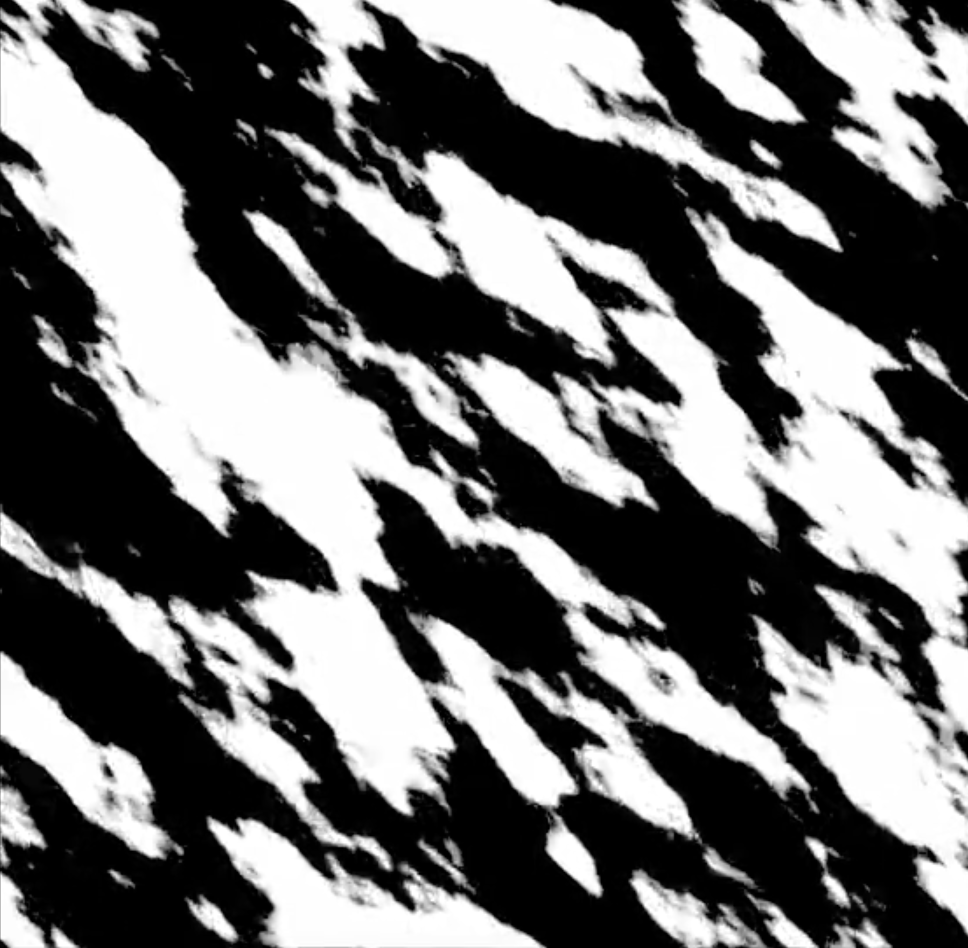
\includegraphics[width=0.3\textwidth]{"images/philips_height_map.png"}
    \captionof{figure}{Height Map using J. Tessendorf's Spectrum}
    \label{fig:tessendorf_height}
\end{minipage}

\vspace{0.3cm}
A significant challenge associated with the utilization of Gerstner waves is the necessity to generate multiple waves for each vertex in order to simulate an ocean. This process can be computationally intensive, particularly considering that an oceanic simulation may be constructed of hundred of thousands vertices. In response to this computational demand, J. Tessendorf (2001) \cite{tessendorf2001} proposed a method for generating ocean waves using the Fourier Transform.

The core concept involves generating a height map of the ocean surface in the frequency domain and converting it back to the time domain using the Inverse Fourier Transform (IFT). The IFT yields a periodic height map, which can be tiled to simulate an infinite ocean surface. This allows us to generate a single texture and apply it across the entire water body.

The benefits of this method are evident when considering a 512x512 texture, which combines 262,144 distinct waves. In contrast, Gerstner waves start to show performance degradation after combining 65 distinct waves for each vertex, which is insufficient for a realistic ocean representation.

To produce the height map, we first need a function that approximates the frequencies. We call this function a spectrum. J. Tessendorf uses a modified Phillips spectrum. This spectrum generates Fourier amplitudes in the frequency domain:
\begin{equation}
    \tilde{h}_0(\mathbf{k}) = \frac{1}{\sqrt{2}}(\xi_r + \xi_i)\sqrt{P_h(\mathbf{k})}
    \label{eq:fouier_amplitudes}
\end{equation}
where $\xi_r$ and $\xi_i$ is a complex number drawn from a Gaussian random number generator with mean 0 and standard deviation 1, $P_h$ is modified Phillips spectrum, and $\mathbf{k}$ is a wave vector.

We then combine $\tilde{h}_0(\mathbf{k})$ with its conjugate $\tilde{h}^{*}_0(-\mathbf{k})$, to "produce waves towards and against the wave direction when propagating"\cite{horvath2015}:
\begin{equation}
    \tilde{h}(\mathbf{k}, t) = \tilde{h}_0(\mathbf{k})e^{i\omega(k)t}+\tilde{h}^{*}_0(-\mathbf{k})e^{-i\omega(k)t}
    \label{eq:combined_amplitudes}
\end{equation}

By performing the Inverse Discrete Fourier Transform (IDFT):
\begin{equation}
    h(\mathbf{x}) = \sum_{\mathbf{k}} \tilde{h}(\mathbf{k}, t)e^{i\mathbf{k}\cdot\mathbf{x}}
    \label{eq:height_map}
\end{equation}
we obtain the height map \ref{fig:tessendorf_height}, where $\mathbf{x}=(x,y)$ represents the position in the texture.

\subsection{Dispersion Relationship}
In the study of wave spectra, it is essential to establish a functional relationship "between the travel speed of waves and their wavelengths", as stated by Christopher J Horvath (2015) \cite{horvath2015}. This relationship, known as the dispersion relation, is typically denoted by $\omega$. In the context of deep water wave dynamics, the dispersion relation is expressed as follows:
$$
\omega^2 = gk
$$
where $g$ is gravity and $k$ denotes the magnitude of the wave vector.

\subsection{Tessendorf's Spectrum}
The appearance of the ocean is largely determined by the spectrum. In his paper, Jerry Tessendorf (2001) \cite{tessendorf2001} proposed a modified version of the Phillips spectrum, which we will refer to as Tessendorf's spectrum. This spectrum takes into account various factors such as the amplitude, wind speed, gravity, and the direction of the waves. However, Tessendorf acknowledges that this spectrum has "poor convergence properties at high values of the wave vectors" \cite{tessendorf2001}.

\subsection{JONSWAP Spectrum}
In response to the challenges experienced with the "Tessendorf's Spectrum", Horvath (2015) \cite{horvath2015} proposed an alternative: the JONSWAP (Joint North Sea Wave Project) spectrum. The spectrum was initially developed by Hasselmann et al. (1973) \cite{hasselmann1973}. This spectrum represents an improvement over the Pierson-Moskowitz Spectrum (1964) \cite{pierson1964}. Hasselmann's key observation was that the wave spectrum is never fully developed. This led him to introduce an extra peak enhancement factor, denoted as $\gamma^r$, into the JONSWAP spectrum.
The JONSWAP spectrum is defined as follows:
\begin{equation}
    \begin{aligned}
        S_{\text{JONSWAP}}(\omega) &= \frac{\alpha g^{2}}{\omega^{5}} \exp \left(-\frac{5}{4} \left(\frac{\omega_{p}}{\omega}\right)^{4}\right) \gamma^{r} \\
        &r = \exp\left(-\frac{(\omega - \omega_p)^{2}}{2 \sigma^{2}\omega^{2}_p}\right) \\
        &\alpha = 0.076 \left( \frac{U^{2}_{10}}{Fg} \right)^{0.22} \\
        &\omega_p = 22 \left( \frac{g^{2}}{U_{10}F} \right)^{1/3} \\
        &\gamma = 3.3 \\
        &\sigma = 
        \begin{cases} 
        0.07 & \text{if } \omega \leq \omega_p \\
        0.09 & \text{if } \omega > \omega_p
        \end{cases}
    \end{aligned}
\end{equation}
where F is the fetch (distance to lee shore), $U_{10}$ is the wind speed at 10 meters above the sea level and $\omega$ is dispersion relationship.

\subsection{The Texel MARSEN ARSLOE (TMA) Spectrum}
One of the limitations of the JONSWAP spectrum is that it only applies to deep waters. To address this, Horvath Christopher \cite{horvath2015} proposed the use of the TMA correction for the deep water spectrum. The TMA was developed by Steven A. Hughes (1984) \cite{hughes1984}, based on observations made by Kitaigordskii (1975) \cite{kitaigordskii1975}. This is known as the Kitaigordskii depth Attenuation function, which is defined as follows:
\begin{equation}
    \begin{aligned}
        \Phi(\omega_h) &= \left[ \frac{(k(\omega, k))^{-3}\frac{\partial k(\omega, h)}{\partial \omega}}{(k(\omega, \infty ))^{-3}\frac{\partial k(\omega, \infty)}{\partial \omega}} \right] \\
        \omega_h &= \omega \sqrt{h/g}
    \end{aligned}
\end{equation}
where $h$ is the depth of the water. At first glance, this function seems complex, but as shown in Figure \ref{fig:tma_correction}, it can be easily approximated.

\begin{minipage}{1\textwidth}
    \centering
    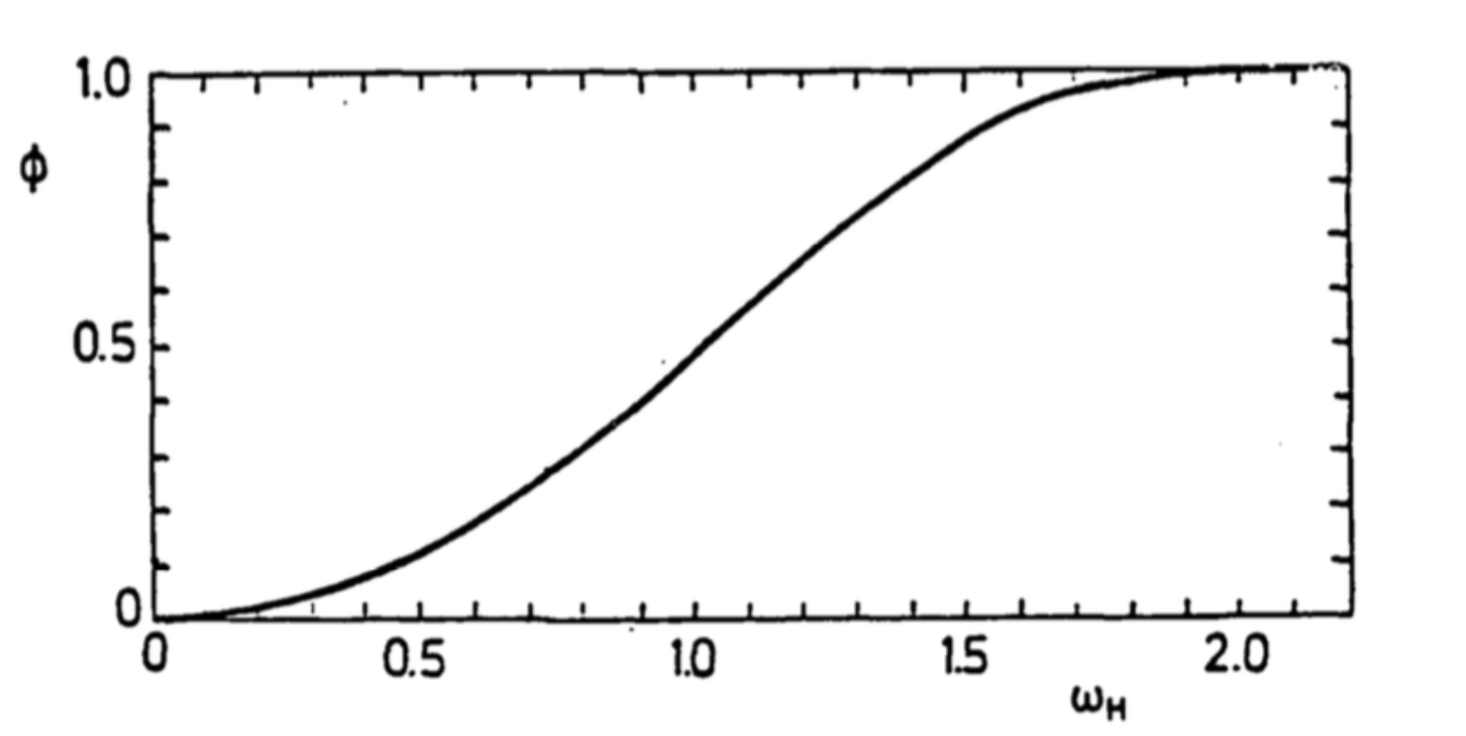
\includegraphics[width=0.45\textwidth]{"images/tma_correction.png"}
    \captionof{figure}{$\Phi(\omega, h)$ as a function of $\omega_h$ \cite{hughes1984}}
    \label{fig:tma_correction}
\end{minipage}

Approximation given by Thomson and Vincent (1983) \cite{thompson1983} is:
\begin{equation}
    \begin{aligned}
        &\Phi(\omega, h) \approx
        \begin{cases} 
        \frac{1}{2} \omega_h^{2} & \text{if } \omega_h \leq 1 \\
        1 - \frac{1}{2}(2 - \omega_h)^{2} & \text{if } \omega_h > 1
        \end{cases}
    \end{aligned}
\end{equation}

With $\Phi(\omega, h)$ we can now correct the JONSWAP spectrum for shallow waters:
\begin{equation}
    S_{\text{TMA}}(\omega, h) = S_{\text{JONSWAP}}(\omega) \Phi(\omega, h)
    \label{eq:tma_spectrum}
\end{equation}

\subsubsection{Donelan-Banner Directional Spreading}
Currently, the TMA spectrum cannot be used for our project due to a few issues. Firstly, this spectrum is non-directional, so we need to add directionality to it. Secondly, this spectrum accepts $\omega$ as input, but as we are following J. Tessendorf's \cite{tessendorf2001} paper, we need to use $\mathbf{k}$ as input.
To solve the first problem Horvath Christopher \cite{horvath2015} proposes to use Donelan-Banner Directional Spreading (1999) \cite{young1999}:
\begin{equation}
    D(\omega, \theta) = \frac{\beta_s}{2 \tanh(\beta_s\pi)}\text{sech}(\beta_s\theta)^{2}
\end{equation}
where,
$$
\begin{aligned}
    &\beta_s =
    \begin{cases} 
    2.61(\omega/\omega_p)^{1.3} & \text{for } 0.56 < \omega/\omega_p < 0.95 \\
    2.28(\omega/\omega_p)^{-1.3} & \text{for } 0.95 \leq \omega/\omega_p < 1.6 \\
    10^{\epsilon} & \text{for } \omega/\omega_p \geq 1.6
    \end{cases}
\end{aligned}
$$
$$
\epsilon = -0.4 + 0.8393 \cdot e^{-0.567\ln(\omega/\omega_p)^{2}}
$$
$$
\theta = \arctan(k.y / k.x) - \theta_{\text{wind}}
$$

In our project we will use $\omega/\omega_p < 0.95$ for first case as it produces more smooth results.
Now we can combine the TMA spectrum with the Donelan-Banner Directional Spreading:
\begin{equation}
    D_{\text{TMA}}(\omega, \theta) = S_{\text{TMA}}(\omega) \cdot D(\omega, \theta)
\end{equation}

\subsubsection{TMA transformation}
Lastly, to make this spectrum usable, we need to transform it from $\omega$ to $\mathbf{k}$ as we follow J. Tessendorf's paper \cite{tessendorf2001}. According to Horvath Christopher \cite{horvath2015}, we can transform it as follows:
\begin{equation}
    S_{\text{TMA}}(\mathbf{k}) = 2S_{\text{TMA}}(\omega, h) \cdot \frac{d\omega}{dk} / k \cdot \Delta k_x \cdot \Delta k_y
    \label{eq:tma_spectrum_k}
\end{equation}
where in our case,
$$
\frac{d\omega}{dk} = \frac{g}{2\sqrt{g*\mathbf{k}}}
$$

\subsection{Cooley-Tukey Fast Fourier Transform (FFT)}
When simulating fourier transform ocean the majority of time is spent on converting from frequency domain to time domain, i.e., performing the IFT.
The previously mentioned IDFT \ref{eq:idft} has time complexity of $O(n^2)$, which is clearly insufficient for simulating higher resolution ocean surfaces in real time.
To address this, the Fast Fourier Transform (FFT) algorithm was invented by Gauss Carl Friedrich (1805) \cite{gauss1866} and later reinvented by Cooley James W. and Tukey John W. (1965) \cite{cooley1965}. 
The FFT algorithm, with a time complexity of $O(n\log n)$, exploits the redundancy in the computation of the DFT to reduce the time complexity. It's important to note that the FFT algorithm only works when the number of samples is a power of 2.

The basic idea of the FFT algorithm is as follows:
\begin{enumerate}
    \item Split the input data into two subsets: one containing the even sample indices and the other containing the odd sample indices. Repeat this process until each subset contains only 2 samples (this is known as bit-reverse sort order).
    \item Generate twiddle factor $W_N = e^{-i 2 \pi k / N}$, raised by k $k$:\\
    \begin{equation}
        k = i * N / 2^{\text{stage} + 1} \text{ mod } N
    \end{equation}
    where $i$ is the index of the sample, stage is the current stage and $N$ is the number of samples.
    \item Perform butterfly operations \ref{fig:butterfly_diagram}, where $x$ and $y$ are complex numbers and $W$ is the twiddle factor

    \begin{minipage}{1\textwidth}
        \centering
        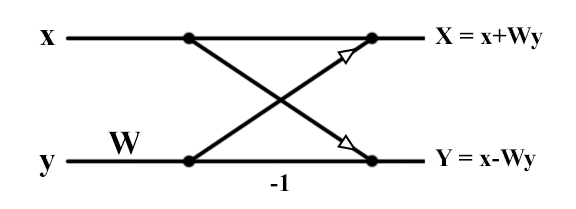
\includegraphics[width=0.4\textwidth]{"images/butterfly_diagram.png"}
        \captionof{figure}{Butterfly Diagram}
        \label{fig:butterfly_diagram}
    \end{minipage}

    \item The butterfly operations are performed in stages \ref{fig:8_butterfly_diagram}. For example, if we have 8 samples, we will have $\log(8) = 3 $ stages. The first stage is for pairs of points (2-point DFTs), the second stage is for groups of four points (4-point DFTs), and so on.
\end{enumerate}

\begin{minipage}{1\textwidth}
    \centering
    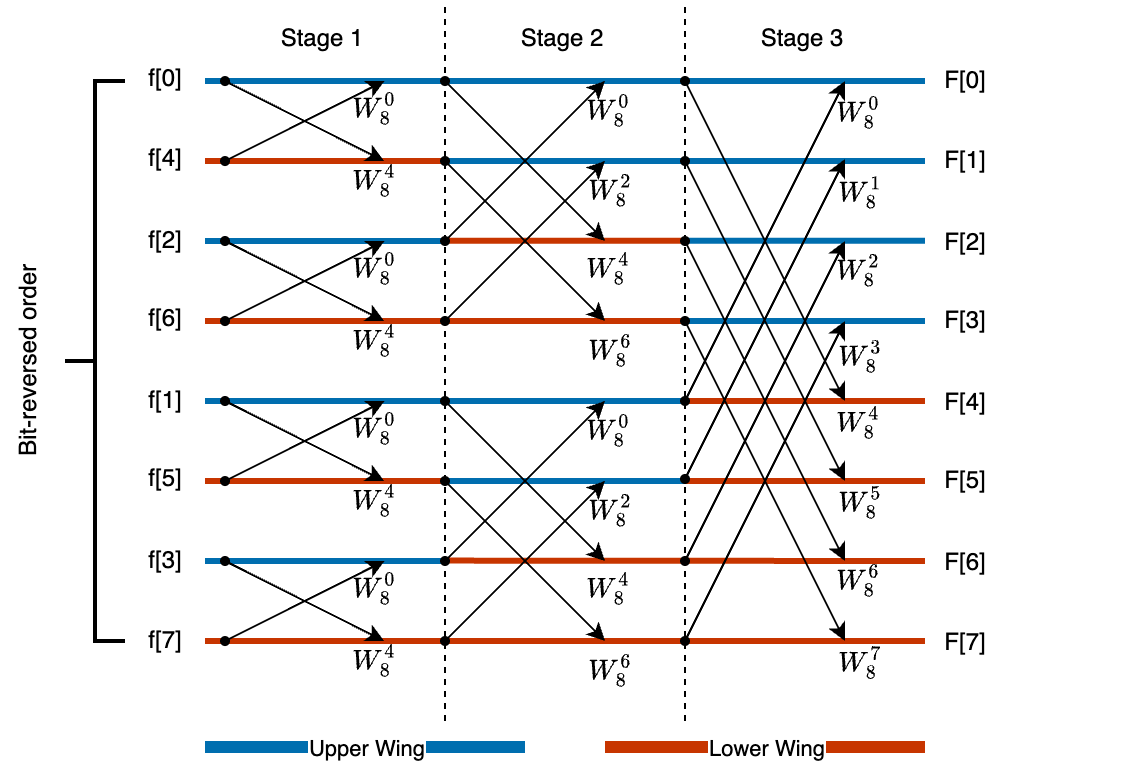
\includegraphics[width=0.7\textwidth]{"images/8_butterfly_diagram.png"}
    \captionof{figure}{8-point FFT Butterfly Diagram}
    \label{fig:8_butterfly_diagram}
\end{minipage}

\subsection{Phong Shading}
The Phong shading model, proposed by Phong Bui Tuong (1975) \cite{phong1975}, is a simple yet effective method for approximating realistic shading. This model consists of three components: ambient shading, diffuse shading, and specular shading, as shown in Figure \ref{fig:phong_shading}.

\begin{minipage}{1\textwidth}
    \centering
    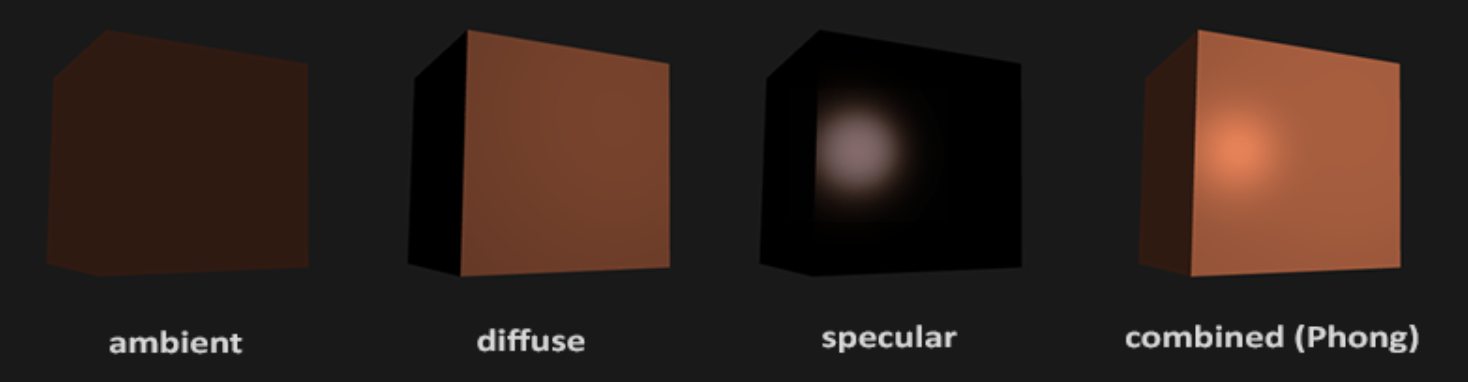
\includegraphics[width=0.6\textwidth]{"images/phong_shading.png"}
    \captionof{figure}{Phong Shading \\ Credits: learnopengl.com}
    \label{fig:phong_shading}
\end{minipage}

The ambient component is a constant value that represents the light scattered throughout the entire scene. The diffuse component can be calculated using the following equation:
\begin{equation}
    \text{Diffuse} = \text{max}(\text{Normal} \cdot \text{LightDirection}, 0.0);
\end{equation}
In this equation, the Normal is a normalized vector that is perpendicular to the surface and points away from it. The specular component can be calculated as follows:
\begin{equation}
    \text{Specular} = max(\text{ViewDir} \cdot \text{ReflectionDir}, 0.0)^{\text{Shininess}}
    \label{eq:phong_specular}
\end{equation}
Here, the ViewDir is a normalized vector pointing towards the camera, and the ReflectionDir is a normalized reflection vector with respect to the Normal. These vectors are illustrated in Figure \ref{fig:phong_graph}.

\begin{minipage}{1\textwidth}
    \centering
    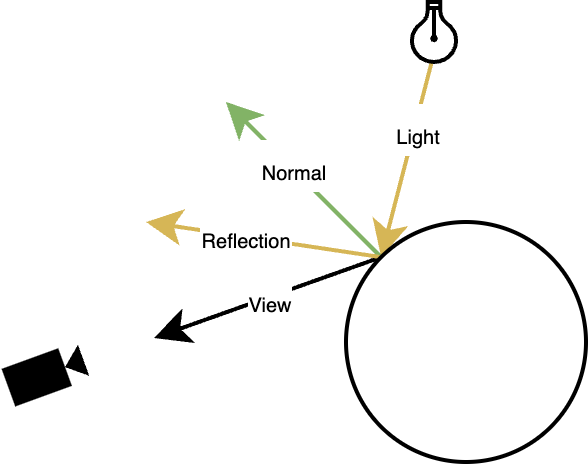
\includegraphics[width=0.4\textwidth]{"images/phong_graph.png"}
    \captionof{figure}{Phong Vectors}
    \label{fig:phong_graph}
\end{minipage}

\subsection{Physically Based Rendering (PBR)}
Earlier mentioned Phong Shading model, does not provide a highly realistic approximation of lighting. To achieve a realistic representation of ocean shading, it is necessary to incorporate a multitude of custom parameters.

Physically Based Rendering (PBR) attempts to address this issue. However, it is important to note that "PBR is more of a conceptual framework than a set of rigid rules" \cite{wilson2017}. The PBR rendering model adheres to three primary principles: energy conservation, microfacet support, and the Fresnel effect.

For the specific application of PBR in ocean shading, one can refer to “Wakes Explosions and Lighting: Interactive Water Simulation in Atlas” by Mark Mihelich and Tim Tcheblokov (2021) \cite{mark2021}, which provides an in-depth discussion on the subject. For a more general understanding of PBR, “Physically Based Shading in Theory and Practice” by Stephen Hill and Stephen McAuley \cite{stephan2012} offers comprehensive coverage of the topic from 2012 to 2020.

\subsection{Particle Simulation and Machine Learning}
Particle-based methodologies, known for their ability to simulate water in a realistic and visually compelling manner, are frequently employed in the field of computer graphics. However, these methods come with a high computational cost, which can be a limiting factor.

Recent advancements in Graphics Processing Unit (GPU) technology have started to alleviate this issue. Research, such as that conducted by Libo Huang et al. (2021) \cite{huang2021}, is making particle simulations increasingly viable for ocean simulation. However, these techniques still demand a high-performance GPU and are not yet suitable for widespread real-time applications.

In addition to these developments, there have been significant strides in the application of machine learning to accelerate fluid simulations. This is evident in the work of Dmitrii Kochkov et al. (2021) \cite{kochkov2021machine}. Despite these advancements, real-time performance on lower-end GPUs remains a challenges which is one of the primary objectives.